\subsection{Особенность иерархической структуры}
Для разработки структурной схемы системы управления мини робота манипулятора была использована иерархическая парадигма архитектуры систем управления роботами. Согласно этой парадигме, иерархическая архитектура системы управления роботом (рис. \ref{Hierar}), в общем случае, содержит четыре уровня управления: интеллектуальный уровень, стратегический уровень, тактический уровень и исполнительный уровень(\citep{Khatib1997}).

\begin{figure}[H]
	\centering
	\includesvg{Src/images/Hierarchy(1).svg}
	\caption{Иерархическая архитектура системы управления роботом}
	\label{Hierar}
\end{figure}

В иерархической архитектуре системы управления роботом манипулятором уровни управления обеспечивают выполнение специфических задач управления роботом:

\begin{itemize}
	\item На интеллектуальном уровне вырабатываются (формируются) решения о выполнении действий роботом манипулятором в условиях неполной информации о внешней среде и объектах, на которые робот воздействует (например, перемещение объекта из одной точки пространства в другую, обработка детали и т.д.).
	\item Стратегический уровень управления предназначен для планирования движений робота манипулятора: разделение задачи действия, выработанной на интеллектуальном уровне, на последовательность согласованных во времени элементарных действий (движений) и формализацию целей управления для каждого из этих действий. Стратегический уровень выдает тактическому уровню план движения в форме команд управления движением. Например, вывод рабочего органа (захватывающего устройства) робота в заданную позицию, захват объекта, тестовое движение для определения сил реакции со стороны объекта, перемещение объекта и возвращение робота в исходную позицию.
	\item На тактическом уровне выполняется преобразование команд управления движением, поступающих со стратегического уровня управления, в программу управления, которая определяет законы согласованного движения во времени всех звеньев робота с учетом технических характеристик блока приводов (в первую очередь ограничений на обобщенные скорости, ускорения и силы). Для выполнения команды позиционного управления движением робота манипулятора на тактическом уровне необходимо определить обобщенные координаты манипулятора, которые соответствуют желаемым декартовым координатам характеристической точки захватывающего устройства робота манипулятора. Для этого решается обратная кинематическая задача о положении манипулятора в заданной точке траектории движения.
	\item Исполнительный уровень управления предназначен для расчета и выдачи управляющих сигналов на блок приводов робота манипулятора в соответствии с программой управления, созданной на тактическом уровне, и с учетом технических характеристик исполнительных устройств.
\end{itemize}

\subsection{Структурная схема системы управления мини робота}

Рисунок \ref{Structural} иллюстрирует структурную схему системы управления мини роботом. Система управления для мини робота манипулятора имеет иерархическую структуру, которая соответствует иерархической архитектуре системы управления роботом (рис. 2.1), так как в разработанной структурной схеме есть устройства, соответствующие функциям уровней управления на (рис.2.1):
\begin{enumerate}
	\item  Устройство стратегического управления (SCD)
	\item  Устройство тактического управления (TCD)
	\item  Устройства исполнительного управления (ACD)
\end{enumerate}

Устройство тактического управления (TCD) мини роботом, координирует работу всех устройств системы управления мини роботом, обеспечивая эффективное функционирование всего механизма робота. Оно выполняет обработку управляющих команд с устройства стратегического управления (SCD) и отвечает за формирование выходных сигналов на устройства исполнительного управления (ACD), обеспечивая соответствие поведения робота с заданными командами.

\begin{figure}[H]
	\centering
	\includesvg[width=\textwidth]{Src/images/Main control system(2).svg}
	\caption{Структурная схема системы управления мини робота}
	\label{Structural}
\end{figure}

Устройство исполнительного управления (ACD) — это устройство, главная цель которого формирование сигналов для точного управления отдельного механического устройства (электродвигателем), обеспечивая поворот плеча робота манипулятора. Данное устройство позволяет выполнять управление двигателем без использования устройства тактического управления (TCD). Благодаря этому можно производить сложные манипуляции с высокой степенью точности и осуществлять поворот осью двигателя на требуемый угол.

После получения данных от устройства стратегического управления (SCD) устройство тактического управления (TCD) отправляет данные на систему управления двигателя каждой из осей (ACD).

После получения команды на движение происходит расчёт позиций, ускорений, а также отправка данных на систему управления движением (ACD) каждой оси. В случае выхода контролируемых параметров за диапазон разрешённых значений улавливается режим аварии и происходит вывод информации на информационную панель.

Панель индикации предоставляет информацию о текущих параметрах и состояний систем, а также о состоянии системы робота. Устройство облегчает мониторинг состояния робота манипулятора и обеспечивает быстрое выявление проблем, путём уведомления оператора. Когда система определяет невозможное дальнейшее движение робота, выполняется индикация красным цветом, цвет ожидания жёлтым, а работу зелёным.

Источник питания является неотъемлемым элементом системы. Так как он, преобразует сетевое электричество, путём формирования значений величины тока и напряжения (24В) до требуемых, для снабжения питанием всех электрических устройств робота. 

Преобразователь напряжения необходим для изменения уровней питающего напряжения до требуемых параметров, так как различные устройства имеют различные значения допустимых параметров питающих напряжений и тока.

Электродвигатели постоянного тока синхронного типа, преобразуют электрическую энергию в механическую. Они обеспечивают движение различных осей робота манипулятора.

Устройство экстренного выключения, используется для мгновенной остановки робота в экстренных ситуациях, предотвращая аварии и повреждения конструкций.

Шина передачи данных обеспечивает коммуникацию между устройством тактического управления (TCD) и устройствами исполнительного управления (ACD). Данная коммуникация позволяет эффективно координировать действия всех устройств управления движением (ACD) между собой, а также производить одновременную синхронизиронизацию во время движения.

\subsection{Структурная схема системы исполнительного управления}

Структурная схема систем управления движением осью изображена на рисунке \ref{ACD}.Назначение данной системы непосредственное управление синхронным двигателем и контроль его параметров. Главными элементами управления системой является устройства исполнительного управления (ACD). Поскольку для управления электродвигателем, необходимы сигналы с регулированием частоты и фазы, и именно   ACD формирует управляющие PWM сигналы.

Драйвера увеличивают мощность управляющих PWM сигналов, тем самым обеспечивая согласование сигнала ACD и выходных силовых транзисторов. Драйверы позволяет производить своевременное и безопасное переключение транзисторов инвертора. 

\begin{figure}[H]
	\centering
	\includesvg[width=\textwidth]{Src/images/Actuator system(1).svg}
	\caption{Структурная схема устройства исполнительного управления}
	\label{ACD}
\end{figure}



Сигналы, подаваемые на электродвигатель, контролируются силовыми ключевыми транзисторами. Электродвигатель необходимо регулировать путем изменения частоты и фазы сигнала

Силовые транзисторы образуют трехфазный мостовой инвертор напряжения и режим работы транзисторов — ключевой. В этом режиме транзисторы переключаются между полностью открытым и полностью закрытым состоянием, это обеспечивает высокий КПД и минимизирует нагрев транзисторов, что особенно важно при создании устройства небольшого размера.

Формирование PWM сигналов выполняется с использованием значений текущего угла поворота оси, ускорения и момента на двигателе. Путем изменения ширины импульсов PWM, система управления ACD может регулировать количество энергии, подаваемой на двигатель, тем самым изменяя параметры скорости и момента.

Преобразователь напряжения, обеспечивает формирование питающих напряжений для различных устройств. Тип преобразователя – DC/DC преобразователь, а преобразуемое напряжения – это напряжение 24В общего источника электропитания. В системе присутствуют различные компоненты с различными уровнями питающего напряжения, поэтому подавать питающее напряжение извне является не эффективным способом.

Шина данных позволяет производить передачу данных между различными устройствами, за счёт соединения компонентов в единую сеть. Благодаря использованию сети появляется возможность производить обмен данными как с одним, так и с несколькими устройствами одновременно. 

\subsection{Алгоритм работы устройства тактического управления}
На рисунке \ref{AlgTCD} изображён главный алгоритм работы устройства тактического управления, главной задачей которого является управление двигателем одной оси робота. По умолчанию, при включении системы, происходит инициализация системы, она подразумевает проверку работоспособности коммуникаций между устройствами и проверку некритического состояния каждого устройства ACD и двигателя. В качестве последнего шага, выполняется инициализация и установка параметров панели индикации.

Если связь с двигателями и интерфейсом управления ACD не нормализовалась, то система управления будет находиться в режиме ожидания до момента восстановления связи. После успешного соединения со всеми устройствами робота происходит установка и отправка команд на исполнительные устройства ACD, минимального значения скорости, угла и ускорения поворота для каждой оси робота. Так как положение осей робота манипулятора после предыдущего выключения неизвестно, необходимо выполнить калибровку всех осей. Калибровка происходит после получения команды разрешения со стороны устройства стратегического управления (SCD).

\begin{figure}[H]
	\centering
	\includesvg[width=\textwidth]{Src/images/Main Controller algorithm.svg}
	\caption{Алгоритм работы устройства тактического управления}
	\label{AlgTCD}
\end{figure}

В варианте работы системы с поднятым флагом включённого состояния робота, после получения соответствующей команды, происходит считывание углов каждой из осей и отправка команд на ACD в зависимости от произведённых вычислений. Таким образом, устройство стратегического управления (SCD) не участвует в расчётах построения пути, а только отправляет данные на устройство тактического управления (TCD).

На изображении \ref{AlgParse} иллюстрируется алгоритм «Parse command». После получения команды со стороны (SCD) происходит выполнение расчёта вида движения.  Расчёт включает в себя набор алгоритмов вида прямолинейного (Move L) и осевого (Move J) движения. В случае получения команд, связанных с действиями робота, например данных об углах поворота или момента каждой из осей, система посылает команду на опрос устройств ACD. Устройство TCD ожидает подтверждения на отосланную команду (ACK command). После этого заканчивается применение алгоритма «Parse command» и происходит переход в «Make calcualtion».

\begin{figure}[H]
	\centering
	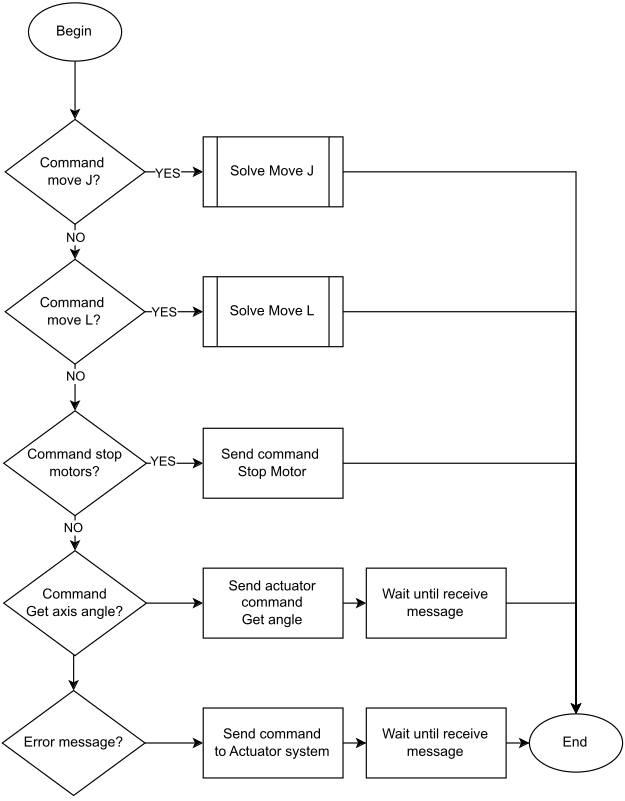
\includegraphics[width=0.8\textwidth]{Src/images/parse.png}
	\caption{Алгоритм «Parse command»}
	\label{AlgParse}
\end{figure}

Основная подпрограмма расчёта траектории движения является, команда "Move J" рисунок \ref{AlgJ}. Основная суть - выполнение движения в определённую позицию более быстрым способом с использованием угловых перемещений. В реализации данной функции происходит расчёт ускорений для каждой оси робота, но только в случае допустимых значений углов планируемой точки. 

\begin{figure}[H]
	\centering
	\includesvg[width=\textwidth]{Src/images/Move J.drawio(1).svg}
	\caption{Алгоритм подпрограммы «Move J»}
	\label{AlgJ}
\end{figure}

Подпрограмма расчёта траектории движения, является командой вычисления линейного движения («Move L», рисунок \ref{AlgL}), руки робота. В наборе алгоритмов выполняется решение обратной задачи, результатом данной задачи является несколько вариантов позиций, углов поворота звеньев робота. Далее требуется требуется формирование списка вариантов позиций робота, которые не будут выходить за границы физических ограничений каждой оси робота. Так же требуется расчёт наименьшего угла от начальной позиции робота.

\begin{figure}[H]
	\centering
	\includesvg[width=\textwidth]{Src/images/Move L.drawio.svg}
	\caption{Алгоритм подпрограммы «Move L»}
	\label{AlgL}
\end{figure}

\subsection{Алгоритм работы устройства исполнительного управления}
Алгоритм устройства исполнительного управления демонстрируется на рисунке \ref{AlgACD}. Данный алгоритм предназначен для управления электродвигателем постоянного тока синхронного типа, который отвечает за поворот управляемой оси робота на определённый угол, и контроля его параметров. 

После включения системы происходит инициализация движения внутренней и внешней периферии. Если инициализация прошла успешно и связь установлена, то происходит проверка необходимости калибровки электродвигателя. Выполнение функции калибровки зависит от набора и значений параметров исполняемой программы. Калибровка необходима, если ось робота подвергалась разборке и было изменено положение устройства измерения угла поворота относительно исходного положения оси.

\begin{figure}[H]
	\centering
	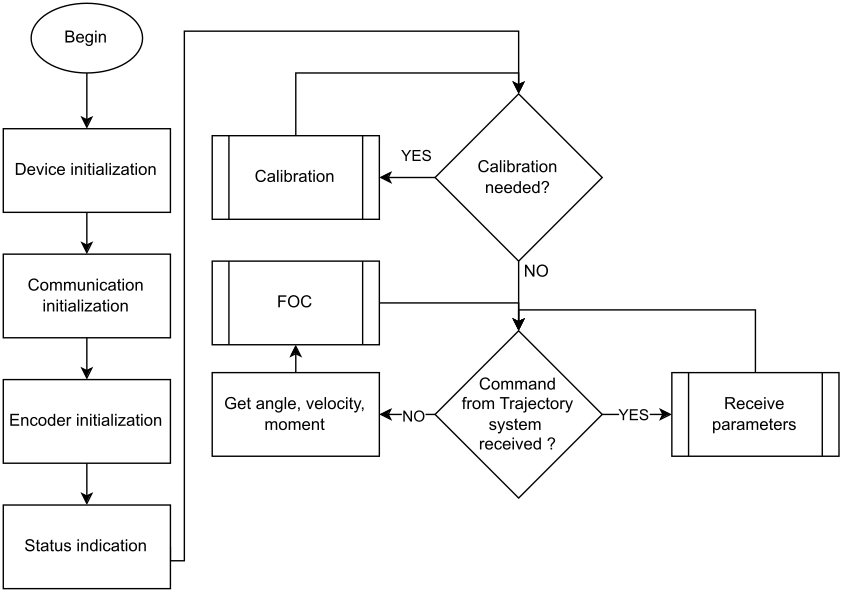
\includegraphics[width=\textwidth]{Src/images/acdalg.png}
	\caption{Алгоритм работы «Actuator control device»}
	\label{AlgACD}
\end{figure}

Далее с определённой периодичностью происходит опрос значений энкодера, которые преобразуются в углы поворота оси двигателя. Данные параметры необходимы в алгоритме расчёта векторного управления. При успешном вычислении параметров векторного управления происходит генерация выходных сигналов на драйвер.

На рисунке \ref{AlgRecive} изображён алгоритм обработки сообщений. Если сообщение от устройства тактического управления (TCD) было получено, то выполняется процесс извлечения, данных из сообщения, которые содержат информацию о необходимой позиции, скорости и коэффициентов регулятора. Данные используются для вычисления параметров векторного регулирования. В случае получения сообщения на запрос данных, производится отправка параметров на устройство отправителя сообщения.

\begin{figure}[H]
	\centering
	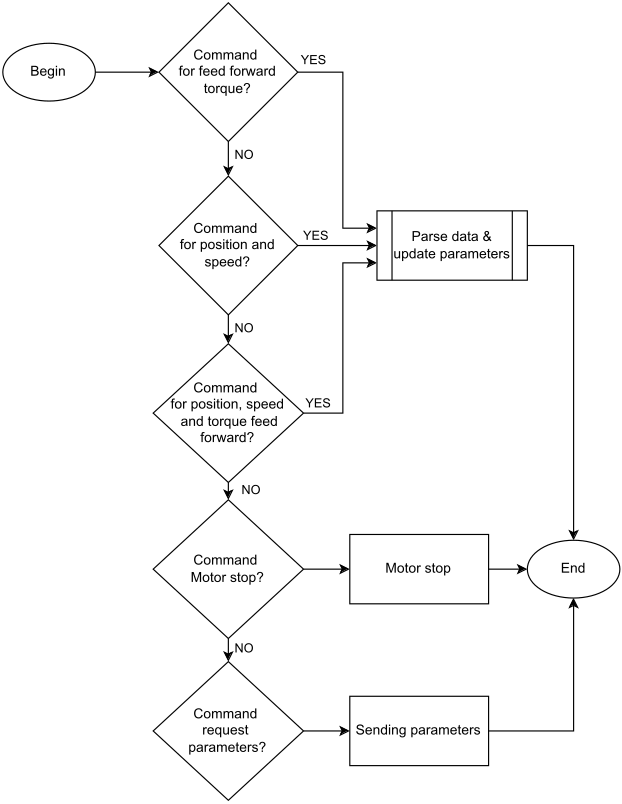
\includegraphics[width=\textwidth]{Src/images/Receive parameters.png}
	\caption{Алгоритм работы подпрограммы «Receive parameters»}
	\label{AlgRecive}
\end{figure}
